\section{119 - K5 - AG 2.2, AG 2.5 - Swing Kitchen - MatKon}

\begin{langesbeispiel} \item[6] %PUNKTE DES BEISPIELS
Seit 2017 gibt es in der Albertgasse mit der "`Swing Kitchen"' ein veganes Fastfoodlokal und da der Großteil der SchülerInnen der 5A sich der \#\! Veganuery-Bewegung angeschlossen hat, verbringen sie also ihre Mittagspause nun meistens in jenem Lokal.

Die Abbildung unten gibt einen Überblick über das Angabot der "`Swing Kitchen"'.
\begin{center}
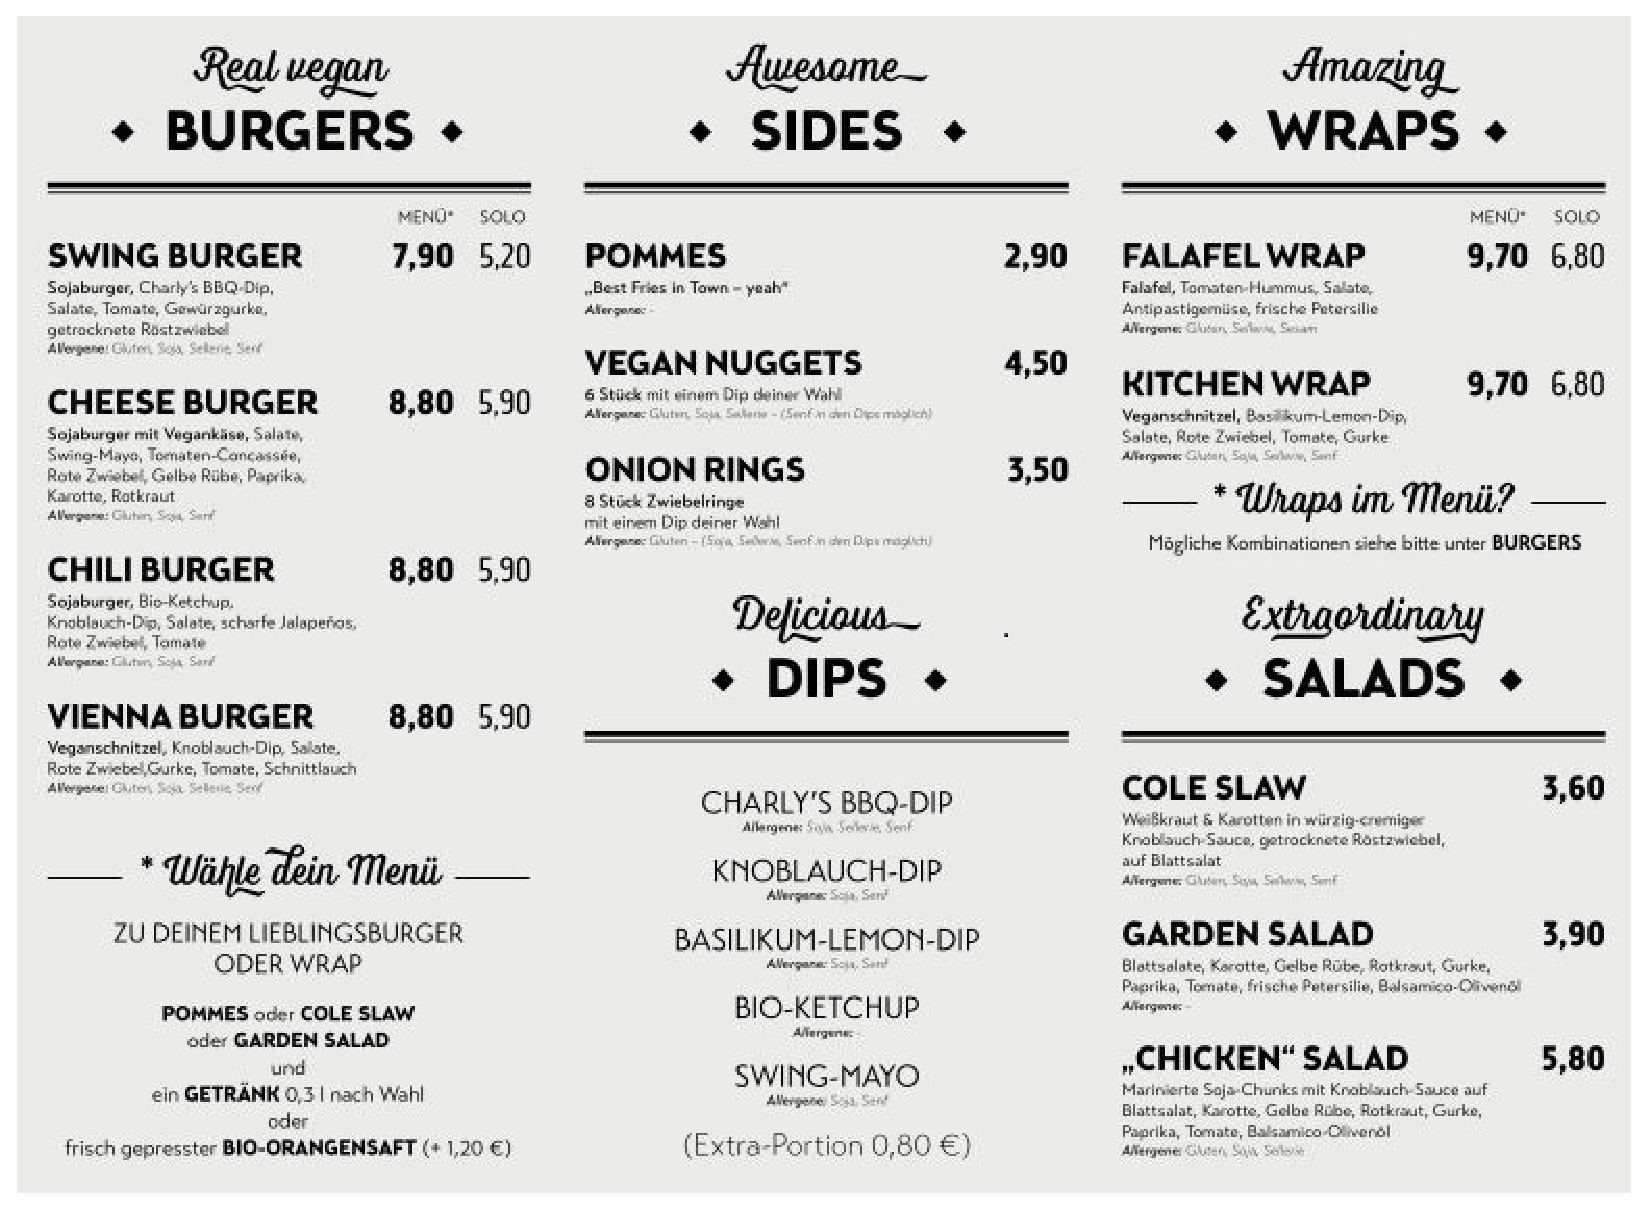
\includegraphics[width=0.8\textwidth]{../_database/Bilder/119_swingkitchen.eps}
\end{center}

Die letzte Bestellung der 5A kann mit folgenden Gleichungen beschrieben werden:
\begin{center}
\begin{tabular}{crcl}
I:&$5,80x+2,90y$&$=$&$92,80$\\
II:&$x$&$=$&$1,5y$\\
\end{tabular}
\end{center}%Aufgabentext

\begin{aufgabenstellung}
\item %Aufgabentext

\Subitem{Interpretiere die Gleichung $5,80x+2,90y=92,80$ im gegebenen Kontext.} %Unterpunkt1
\Subitem{Interpretiere die Gleichung $x=1,5y$ im gegebenen Kontext.} %Unterpunkt2

\item %Aufgabentext

\ASubitem{Löse das Gleichungssystems.} %Unterpunkt1
\Subitem{Interpretiere die Lösung im gegebenen Kontext.} %Unterpunkt2

\item %Aufgabentext

\Subitem{Finde für die erste Gleichung drei andere Lösungspaare.} %Unterpunkt1
\Subitem{Zeige rechnerisch, dass es sich bei den drei Lösungen um keine Lösungen der zweiten Gleichung handelt.} %Unterpunkt2

\end{aufgabenstellung}

\begin{loesung}
\item \subsection{Lösungserwartung:} 

\Subitem{Die 5A hat x-mal einen Chicken-Salad und y-mal Pommes bestellt und musste dafür 92,80\,\euro zahlen.} %Lösung von Unterpunkt1
\Subitem{Die 5A hat 1,5-mal mehr Chicken-Salads gekauft als Pommes.} %%Lösung von Unterpunkt2

\setcounter{subitemcounter}{0}
\subsection{Lösungsschlüssel:}
 
\Subitem{Ein Punkt für die richtige Interpretation der ersten Gleichung.} %Lösungschlüssel von Unterpunkt1
\Subitem{Ein Punkt für die richtige Interpretation der zweiten Gleichung.} %Lösungschlüssel von Unterpunkt2

\item \subsection{Lösungserwartung:} 

\Subitem{$5,80\cdot 1,5y+2,90y=92,80\quad\Rightarrow\quad 11,6y=92,80\quad\Rightarrow\quad y=8\quad\Rightarrow\quad x=12$} %Lösung von Unterpunkt1
\Subitem{Die 5A hat 12 mal Chicken-Salad und 8 mal Pommes bestellt.} %%Lösung von Unterpunkt2

\setcounter{subitemcounter}{0}
\subsection{Lösungsschlüssel:}
 
\Subitem{Ein Punkt für die richtige Berechnung des Schnittpunkts.} %Lösungschlüssel von Unterpunkt1
\Subitem{Ein Punkt für die richtige Interpretation des Schnittpunkts.} %Lösungschlüssel von Unterpunkt2

\item \subsection{Lösungserwartung:} 

\Subitem{Mögliche Lösungen:\\
$(0\mid 32)$, $(16\mid 0)$, $(6\mid 20)$} %Lösung von Unterpunkt1
\Subitem{Mögliche Vorgehensweise:\\
$0\neq 1,5\cdot 32$, $16\neq 1,5\cdot 0$, $6\neq 1,5\cdot 20$} %%Lösung von Unterpunkt2

\setcounter{subitemcounter}{0}
\subsection{Lösungsschlüssel:}
 
\Subitem{Ein Punkt für die Angabe von zwei Lösungspaare.} %Lösungschlüssel von Unterpunkt1
\Subitem{Ein Punkt für die Angabe eines dritten Lösungspaars.} %Lösungschlüssel von Unterpunkt2

\end{loesung}

\end{langesbeispiel}